%!TEX root = thesis.tex

\chapter{Introduction}
\label{sec:introduction}

Bacon ipsum dolour sit amet porchetta beef turkey, bacon turducken boudin hamburger venison ball tip. Brisket pork loin bresaola short loin ground round leberkas pastrami tongue jerky cow turducken beef ribs. Pork ribeye landjaeger prosciutto pig venison tenderloin. Swine beef ribs kielbasa, porchetta tenderloin salami venison pork belly tail.

\section{Figures}

\begin{figure}
  \centering
  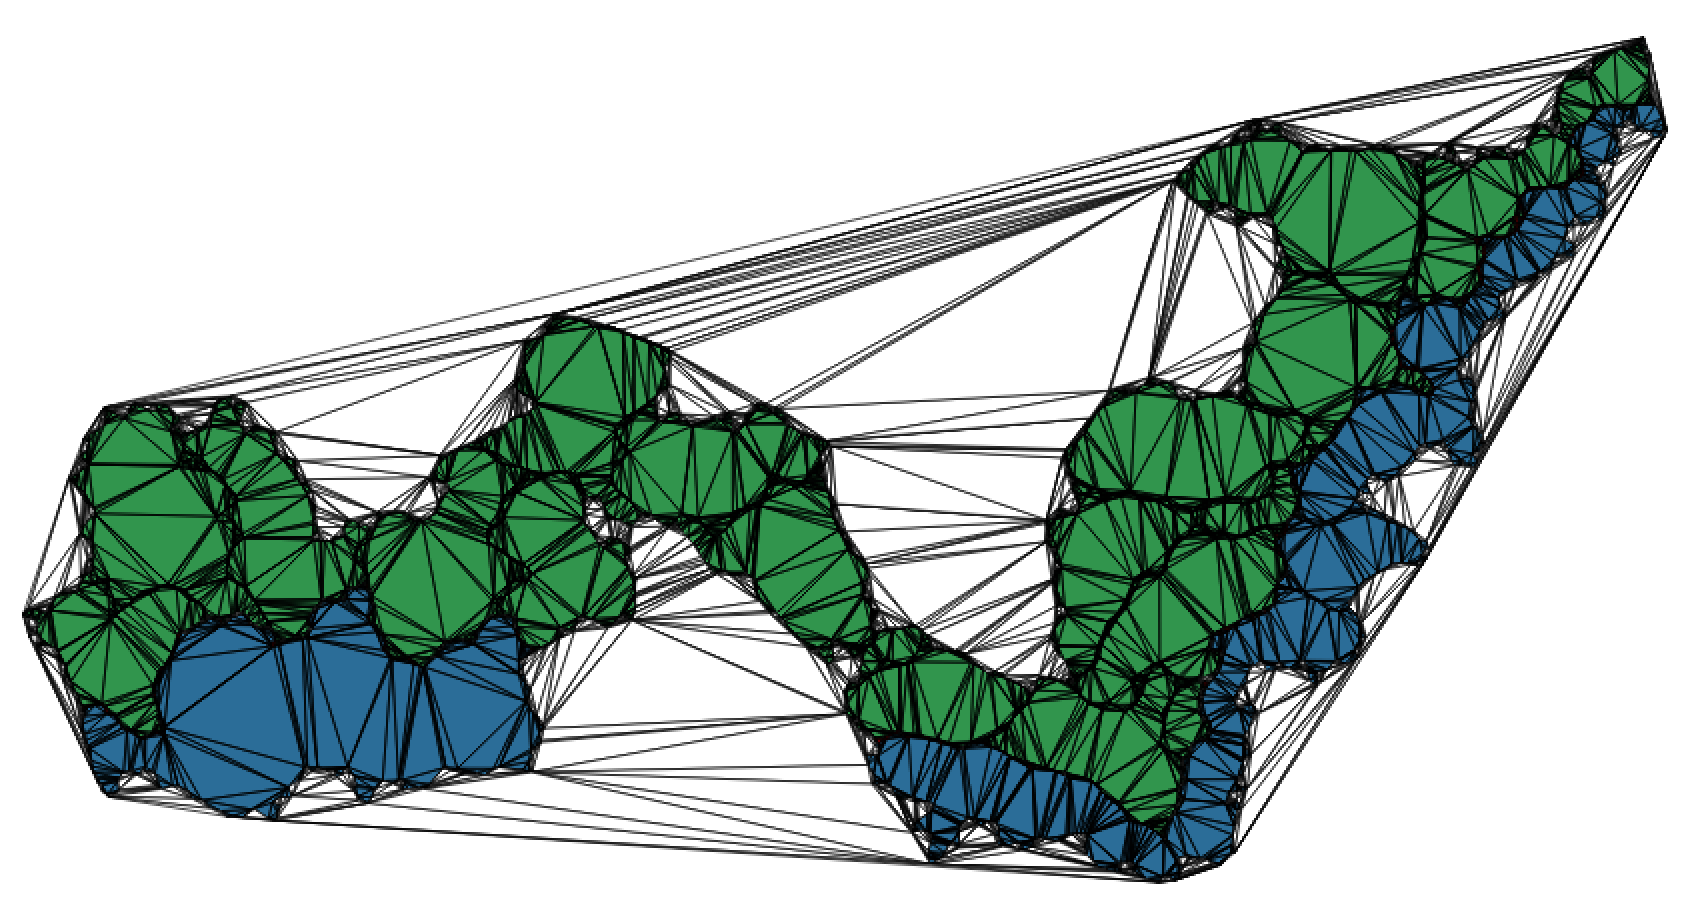
\includegraphics[width=0.8\linewidth]{figs/sometriangles.png}
  \caption{One nice figure}
\label{fig:sometriangles}
\end{figure}

As shown in Figure~\ref{fig:sidebyside},
\begin{figure}
  \centering
  \begin{subfigure}[b]{0.45\linewidth}
    \centering
    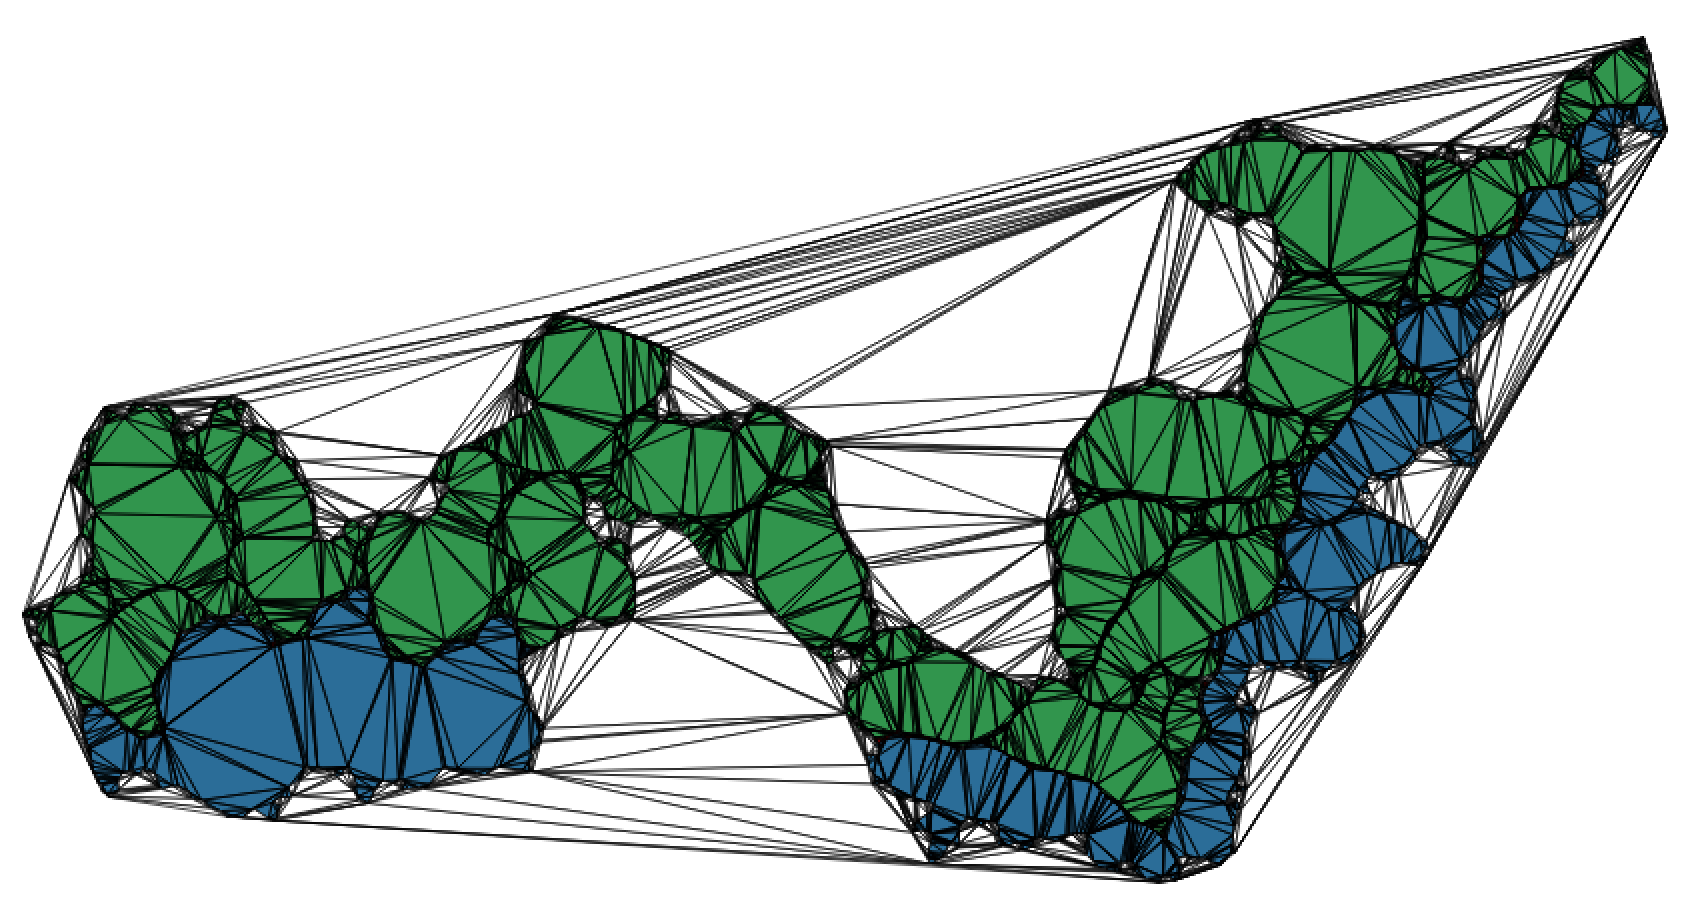
\includegraphics[width=\linewidth]{figs/sometriangles.png}
    \caption{}\label{fig:sidebyside:1}
  \end{subfigure}%
  \qquad %-- that adds some space between th 2 figures
  \begin{subfigure}[b]{0.45\linewidth}
    \centering
    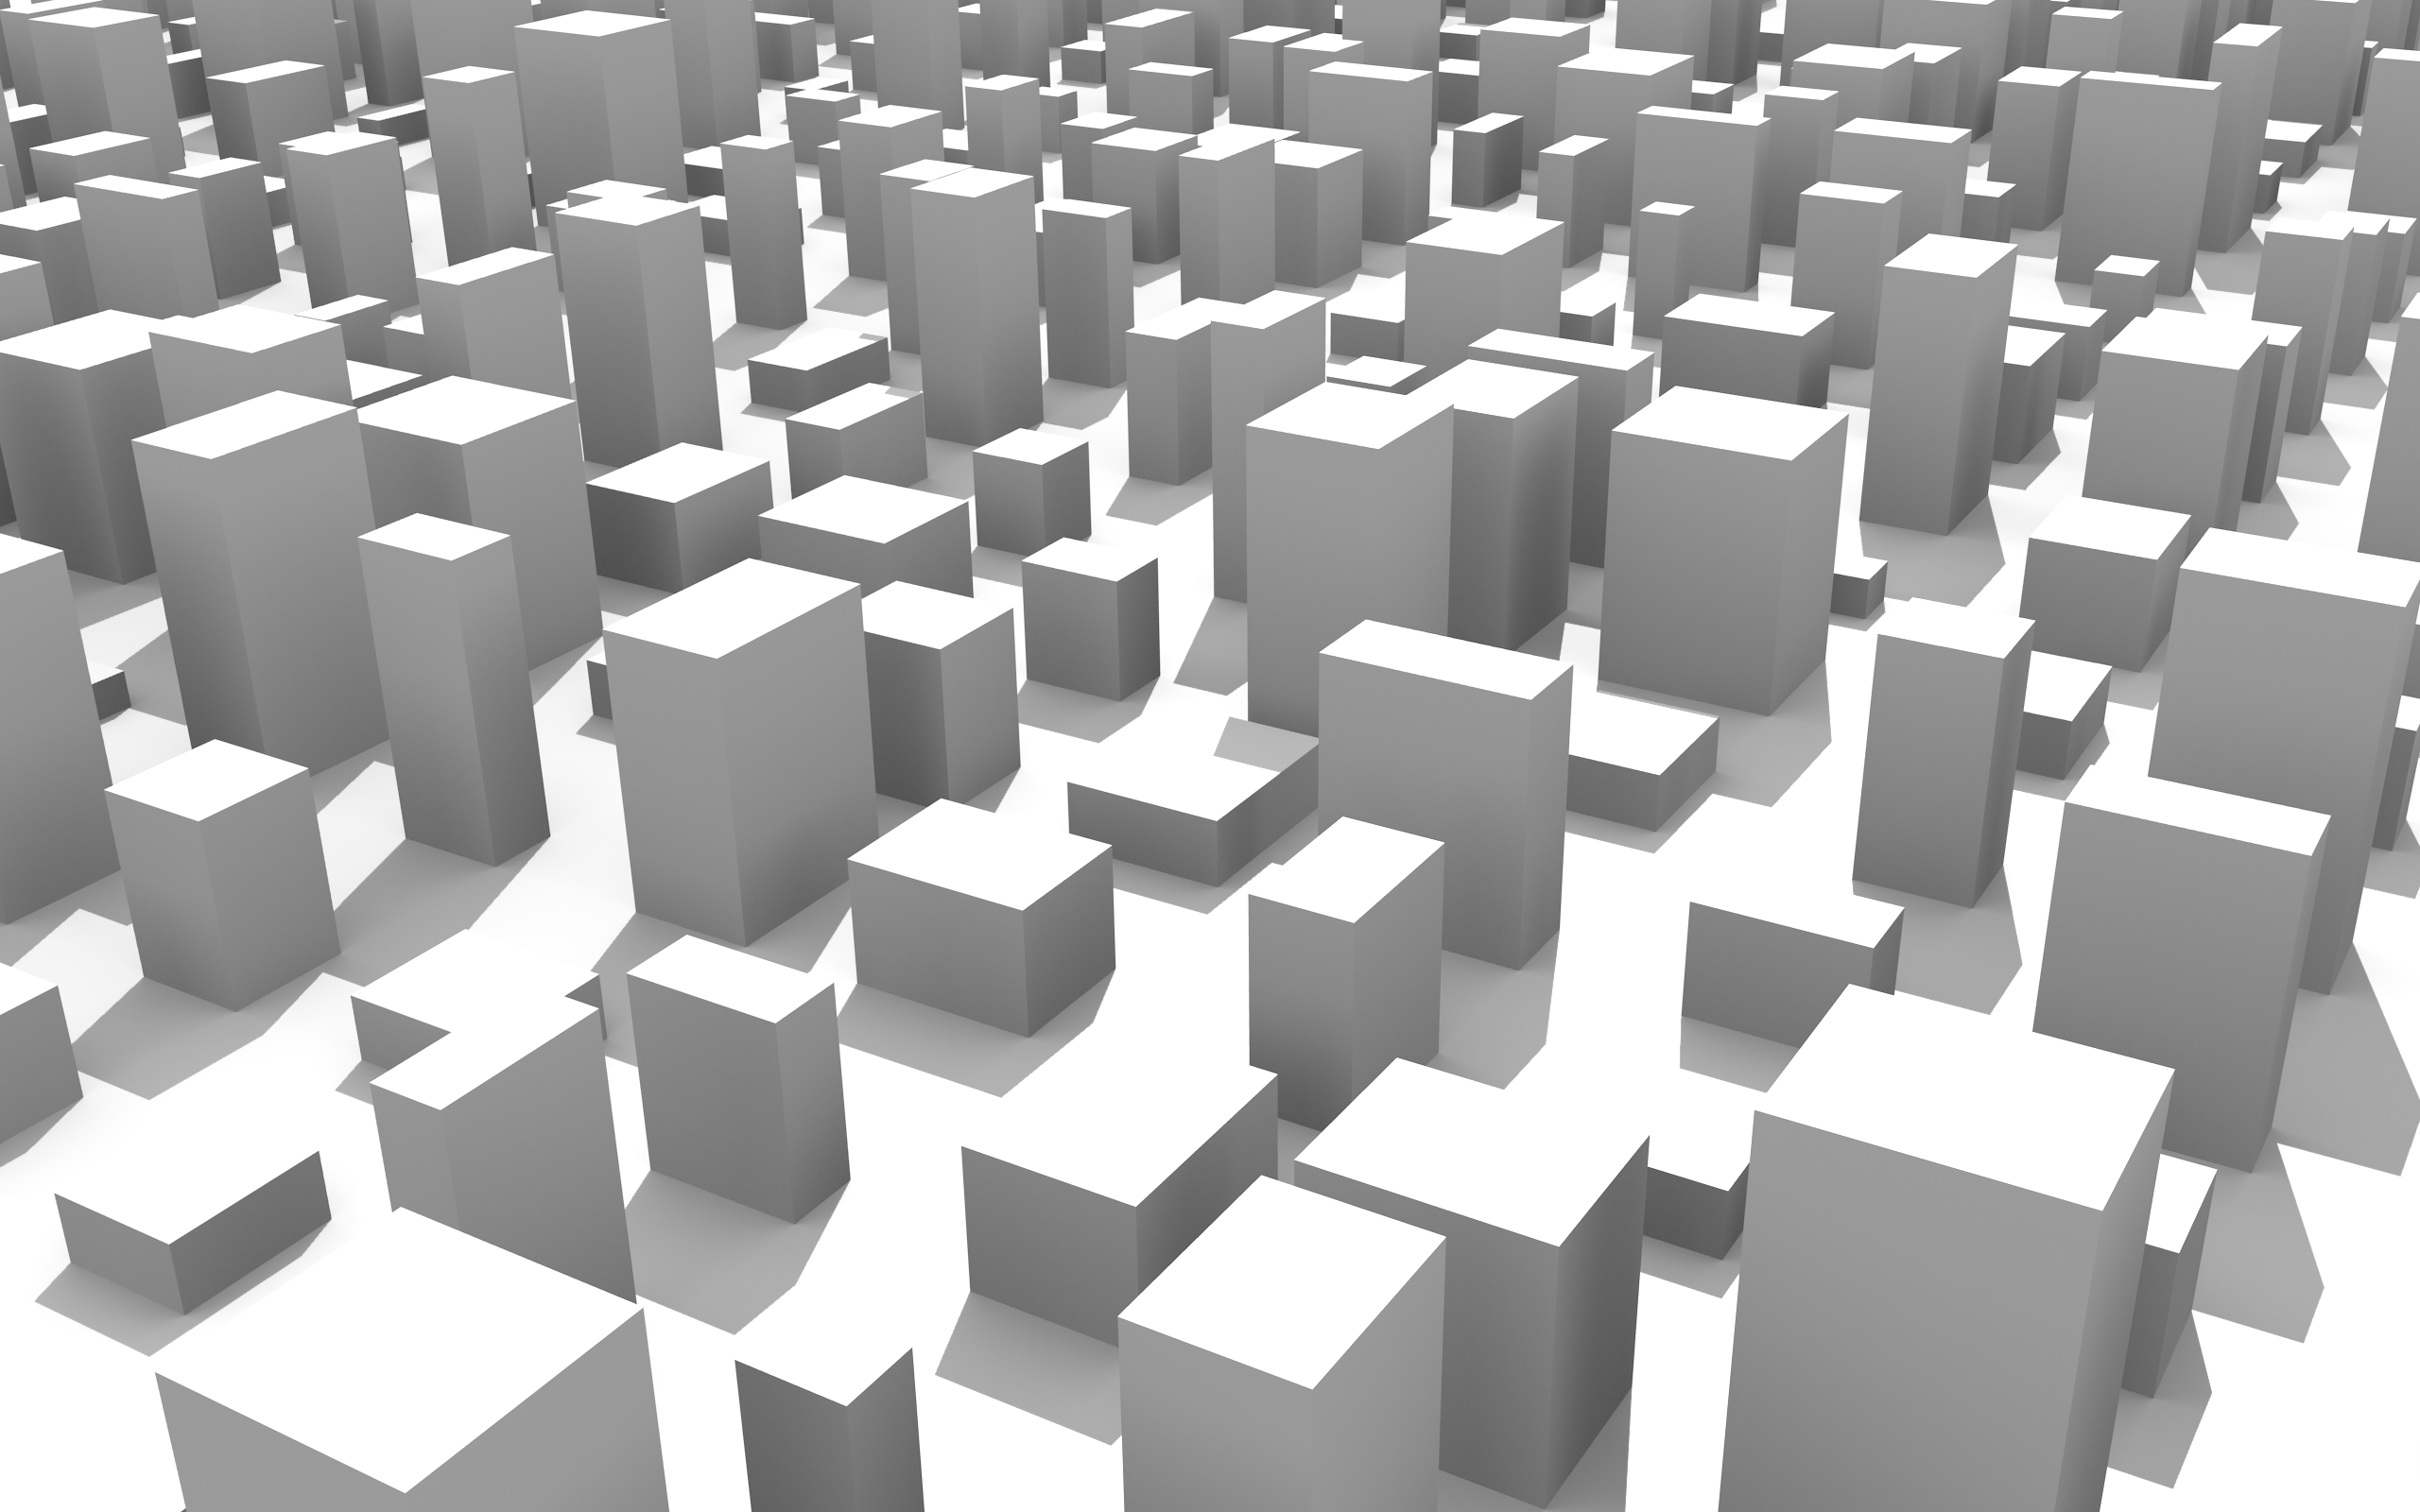
\includegraphics[width=\linewidth]{figs/lod1.png}
    \caption{}\label{fig:sidebyside:2}
  \end{subfigure}%
  \caption{Two figures side-by-side.}\label{fig:sidebyside}
\end{figure}
it is possible to have two figures (or more) side by side.
You can also refer to a subfigure: see Figure~\ref{fig:sidebyside:2}.


\subsection{Figures in PDF are possible (and better)}

If you use Adobe Illustrator or Ipe you can make your figures vectorial and save them in PDF\@.
You include a PDF the same way as you do for a PNG, see Figure~\ref{fig:pdffig},
\begin{figure}
  \centering
  \begin{subfigure}[b]{0.2\linewidth}
    \centering
    
\includegraphics[page=1,width=\linewidth]{figs/tricat.pdf}
    \caption{}\label{fig:pdffig:1}
  \end{subfigure}%
  \qquad %-- that adds some space between th 2 figures
  \begin{subfigure}[b]{0.2\linewidth}
    \centering
    
\includegraphics[page=2,width=\linewidth]{figs/tricat.pdf}
    \caption{}\label{fig:pdffig:2}
  \end{subfigure}%
  \qquad %-- that adds some space between th 2 figures
  \begin{subfigure}[b]{0.2\linewidth}
    \centering
    
\includegraphics[page=3,width=\linewidth]{figs/tricat.pdf}
    \caption{}\label{fig:pdffig:3}
  \end{subfigure}%
  \caption{Three PDF figures side-by-side.}\label{fig:pdffig}
\end{figure}



\section{How to add references?}

\citet{Descartes37} wrote and another one too~\citep{Voronoi08,Delaunay34}.


\section{Pseudo-code}

Please try to not put code in a thesis, instead put pseudo-code.
The package \texttt{algorithm2e} is pretty handy, see for instance the Algorithm~\ref{alg:myfirst}.
\begin{algorithm}[h]
 \KwData{this text}
 \KwResult{how to write algorithm with \LaTeX2e }
 initialization\;
 \While{not at end of this document}{
  read current\;
  \eIf{understand}{
   go to next section\;
   current section becomes this one\;
   }{
   go back to the beginning of current section\;
  }
 }
 \caption{How to write algorithms}\label{alg:myfirst}
\end{algorithm}
All your algorithms will be automatically added to the list of algorithms at the begining of the thesis.
